\documentclass[12pt,a4paper]{article}

% --- Language & Encoding Packages ---
\usepackage{iftex}
\ifPDFTeX
  \usepackage[utf8]{inputenc}
  \usepackage[english]{babel}
  \usepackage[T1]{fontenc}
\else
  \usepackage{fontspec}
  \usepackage[english]{babel}
\fi

% --- Page Layout & Geometry ---
\usepackage[top=2.5cm,bottom=2.5cm,left=2.5cm,right=2.5cm]{geometry}
\usepackage{setspace}
\onehalfspacing

% --- Graphics, Figures & Colors ---
\usepackage{graphicx}
\usepackage{xcolor}
\usepackage{float}
\usepackage{tikz}
\usetikzlibrary{shapes.geometric, arrows, positioning, fit, backgrounds, calc}

% --- Math & Formulas ---
\usepackage{amsmath,amssymb}

% --- Code Listings & Highlighting ---
\usepackage{listings}
\definecolor{codegreen}{rgb}{0,0.6,0}
\definecolor{codegray}{rgb}{0.5,0.5,0.5}
\definecolor{codepurple}{rgb}{0.58,0,0.82}
\definecolor{backcolour}{rgb}{0.96,0.97,0.98}
\definecolor{deepblue}{rgb}{0.0,0.2,0.6}

\lstdefinestyle{codeStyle}{
    backgroundcolor=\color{backcolour},
    commentstyle=\color{codegreen},
    keywordstyle=\color{deepblue}\bfseries,
    numberstyle=\tiny\color{codegray},
    stringstyle=\color{codepurple},
    basicstyle=\ttfamily\footnotesize,
    breakatwhitespace=false,
    breaklines=true,
    captionpos=b,
    keepspaces=true,
    numbers=left,
    numbersep=6pt,
    showspaces=false,
    showstringspaces=false,
    showtabs=false,
    tabsize=2,
    frame=single,
    rulecolor=\color{black!20}
}
\lstset{style=codeStyle}

\lstdefinelanguage{json}{
    basicstyle=\ttfamily\footnotesize,
    numbers=left,
    numberstyle=\tiny\color{codegray},
    stepnumber=1,
    numbersep=6pt,
    showstringspaces=false,
    breaklines=true,
    frame=single,
    backgroundcolor=\color{backcolour}
}

% --- Tables & Enums ---
\usepackage{booktabs}
\usepackage{array}
\usepackage{tabularx}
\usepackage{enumitem}

% --- Table of Contents & Numbering Depth ---
\setcounter{tocdepth}{3}
\setcounter{secnumdepth}{3}

% --- Header & Footer ---
\usepackage{fancyhdr}
\setlength{\headheight}{15pt}
\pagestyle{fancy}
\fancyhf{}
\rhead{\small\textit{CS426 -- Mobile Application Development}}
\lhead{\small\textit{Personal Document -- Project Report}}
\cfoot{\thepage}

% --- Hyperlinks ---
\usepackage{hyperref}
\hypersetup{
    colorlinks=true,
    linkcolor=deepblue,
    filecolor=magenta,      
    urlcolor=cyan,
    pdftitle={Final Project Report - Personal Document},
    pdfpagemode=FullScreen,
}

% --- Title Information ---
\title{
    \vspace{-1.5cm}
    \textbf{\Large VIETNAM NATIONAL UNIVERSITY HO CHI MINH CITY}\\
    \textbf{\large UNIVERSITY OF SCIENCE -- FACULTY OF INFORMATION TECHNOLOGY}\\
    \vspace{1cm}
    \textbf{\LARGE FINAL PROJECT REPORT}\\[0.3cm]
    \textbf{\Large COURSE: MOBILE APPLICATION DEVELOPMENT (CS426)}\\[0.6cm]
    \textbf{\huge \color{deepblue} PERSONAL DOCUMENT}\\[0.3cm]
    \textit{\large An Intelligent On-Device Personal Document Management and Search Application}\\
    \textit{\normalsize Cloud-First Architecture with Resilient On-Device Local Fallback}
    \vspace{0.8cm}
}

\author{
    \textbf{Project Members:} \\
    Trinh Nam Kiet -- \texttt{Student ID: CS426} \\
    Doan Tuan Anh -- \texttt{Student ID: CS426} \\
    \vspace{0.5cm} \\
    \textbf{Instructors:} \\
    Department of Software Engineering
}

\date{September 2026}

\begin{document}

\begin{titlepage}
    \newcommand{\HRule}{\rule{\linewidth}{0.5mm}}
    \centering

    \textsc{\LARGE Vietnam National University Ho Chi Minh City}\\[0.4cm]
    \textsc{\Large University of Science}\\[0.4cm]
    \textsc{\large Faculty of Information Technology}\\[0.6cm]
    \textsc{Department of Software Engineering}\\[0.6cm]

    \HRule{}\\[0.5cm]
    {\huge\bfseries PERSONAL DOCUMENT}\\[0.3cm]
    {\large\bfseries Final Project Report}\\[0.4cm]
    \HRule{}\\[0.8cm]

    \textbf{\large Course: Mobile Application Development (CS426)}\\[1.0cm]

    \begin{center}
        \large
        \textit{Project members:}\\[0.4cm]
        Trinh Vo Nam Kiet -- 24125013\\
        Doan Tuan Anh -- 24125002\\
        Tran Khanh Nhan -- 24125037
    \end{center}
    \vspace{1.2cm}

    \includegraphics[scale=0.18]{/home/namkiet/Desktop/hcmus/mobile/midterm/report/images/hcmus-logo.png}\vspace{1.2cm}

    {\large September 2026}\\[1cm]
    \vfill
\end{titlepage}

\newpage
\setcounter{tocdepth}{3}
\tableofcontents
\newpage

\subsection*{Work Division}
\begin{table}[H]
\centering
\small
\begin{tabularx}{\textwidth}{l p{3.2cm} X}
\toprule
\textbf{Student ID} & \textbf{Full Name} & \textbf{Main Responsibilities} \\
\midrule
24125013 & Trinh Vo Nam Kiet & Implemented the offline document-processing workflow, including OCR-based metadata generation, object detection, and local embedding-based search. \\
24125002 & Doan Tuan Anh & Implemented the online Gemini-based processing pipeline, OCR and detection integration, and AI-assisted document analysis. \\
24125037 & Tran Khanh Nhan & Designed and implemented the application UI, including the main screens, navigation flow, and data models used across the app. \\
\bottomrule
\end{tabularx}
\caption{Work division among project members}
\end{table}

\newpage

% --- Section Content Inputs ---
\section{Project Overview}

\subsection{Course Context and Application}
The \textbf{Personal Document} project is developed as the capstone final project for the course \textbf{Mobile Application Development (CS426)} at the University of Science, Vietnam National University Ho Chi Minh City (HCMUS).

\textbf{Personal Document} is a native Android application (supporting Android 7.0, API Level 24 and higher, built entirely with Kotlin, Jetpack Compose, Material Design 3, Room, MediaPipe, ML Kit, and Coroutines/Flow). The application functions as an intelligent personal digital repository, empowering users to digitize, automatically analyze, structure, and search through photo-captured documents, receipts, study notes, and personal credentials.

\subsection{Problem Statement and User Pain Points}
In our fast-paced daily study and professional lives, the smartphone camera has naturally evolved into our primary instantaneous memory capture tool:
\begin{itemize}
    \item \textbf{Students} snap photos of lecture slides, whiteboard derivations, textbook excerpts, and handwritten peer study notes.
    \item \textbf{Working professionals and freelancers} photograph dining receipts, fuel bills, travel invoices for expense reimbursement, client contracts, and business cards.
    \item \textbf{Everyday individuals} capture citizen IDs, health insurance cards, medical prescriptions, home appliance warranties, and utility meter readings.
\end{itemize}

\paragraph{The Everyday User Dilemma:}
Imagine standing at a government administrative office or facing the monthly company expense audit deadline. You distinctly recall photographing a business lunch receipt or an insurance policy card three weeks ago. You open your default system Gallery app. Immediately, you are confronted with a disorganized labyrinth of thousands of photos: holiday snapshots, food photos, selfies, downloaded memes, social media screenshots, and family videos.

The filenames offer no assistance, represented merely by arbitrary computer-generated timestamps such as \texttt{IMG\_20260905\_143022.jpg}. You find yourself scrolling endlessly, squinting through hundreds of tiny thumbnails, desperate to locate that single piece of paper. This process easily squanders 10 to 15 minutes of frustration, and in many instances, users give up entirely, forfeiting financial reimbursement or missing critical deadlines.

\paragraph{Core Limitations of Existing Solutions:}
\begin{enumerate}
    \item \textbf{Visual Pollution and Document Fragmentation:} Critical documents are dumped alongside casual photos in the device gallery, lacking any dedicated workspace.
    \item \textbf{Primitive Search Capabilities:} Traditional mobile galleries index media solely by timestamp or rough GPS location. When a user remembers the conceptual contents (e.g., \textit{"Phuc Long coffee invoice"} or \textit{"B-Tree database index slide"}), system galleries remain entirely helpless.
    \item \textbf{Heavy Manual Data Entry Friction:} Conventional scanning and note-taking apps require users to manually type titles, select categories, and compose tags. This tedious overhead causes cognitive friction, discouraging consistent organizational habits.
    \item \textbf{Privacy Concerns and Network Dependence:} Cloud-exclusive document scanners upload sensitive personal and financial credentials to third-party servers, posing serious data privacy risks and rendering the application useless during cellular dead zones or offline travel.
\end{enumerate}

\subsection{Proposed Solution}
\textbf{Personal Document} directly addresses these challenges by merging an adaptive \textbf{Cloud-First} architecture with a dependable \textbf{Offline On-Device Machine Learning} pipeline:
\begin{itemize}
    \item \textbf{Isolated, Private Repository:} Scanned and imported documents are organized in an app-private library, completely segregated from everyday media in the Android system gallery.
    \item \textbf{Automated Metadata Generation Pipeline:} The moment an image is captured or selected, the system autonomously:
    \begin{itemize}
        \item Transcribes all text via optical character recognition (OCR).
        \item Identifies visible real-world objects through image labeling.
        \item Generates a concise title, a single-sentence descriptive summary, predicts the appropriate category (\textit{NOTE, RECEIPT, IDENTITY, STUDY, WORK, OTHER}), and suggests up to 5 topical tags.
    \end{itemize}
    \item \textbf{Human-in-the-Loop Verification:} All AI-generated fields are treated strictly as suggestions encapsulated within a \texttt{DocumentDraft}. Users inspect and can freely modify any field on an interactive Review screen before confirming persistence.
    \item \textbf{Fuzzy Hybrid Search Engine:} The application combines semantic vector similarity (cosine similarity over 512-dimensional embeddings) with typo-tolerant lexical matching (Levenshtein distance). Users can locate documents via conceptual queries or misspelled keywords effortlessly.
    \item \textbf{Cloud-First with Resilient Local Fallback:} The application defaults to Google's Gemini Vision API when online for maximum multimodal reasoning, but gracefully falls back to local Google ML Kit and MediaPipe on-device models when offline or if disabled by user settings.
\end{itemize}

\section{Project Scope}

\subsection{Target Users}
The application is specifically engineered for several distinct user demographics:
\begin{enumerate}
    \item \textbf{Students, Researchers, and Educators:}
    \begin{itemize}
        \item Frequently capture lecture slides, whiteboard solutions, textbook diagrams, academic papers, and homework sheets.
        \item Require systematic categorization under the \textit{STUDY} domain and rapid retrieval of formulas, definitions, or exam topics during revision.
    \end{itemize}
    \item \textbf{Office Workers, Freelancers, and Small Business Owners:}
    \begin{itemize}
        \item Need to capture, track, and aggregate commercial receipts, meal vouchers, travel tickets, and invoices for monthly financial accounting and expense claims (\textit{RECEIPT}).
        \item Organize project plans, meeting agendas, physical business cards, and signed contracts under the \textit{WORK} category.
    \end{itemize}
    \item \textbf{Everyday Individuals and Household Organizers:}
    \begin{itemize}
        \item Maintain crucial personal identification credentials such as National IDs, Passports, Driver's Licenses, and Medical Insurance Cards (\textit{IDENTITY}).
        \item Individuals prone to forgetfulness who benefit from an intelligent search engine that understands conceptual context rather than requiring exact keyword memory.
    \end{itemize}
\end{enumerate}

\subsection{Target Platform}
\begin{itemize}
    \item \textbf{Operating System:} Native Android OS, with full backward compatibility spanning from \textbf{Android 7.0 (API Level 24 -- Nougat)} up to the latest releases (\textbf{Android 14 and 15}).
    \item \textbf{Hardware Requirements:} Designed to execute efficiently on mid-range and budget Android smartphones (requiring a minimum of 3GB to 4GB of RAM and a standard autofocus rear camera module for clear optical capture).
    \item \textbf{Operating Environment:} Built to perform seamlessly in dual operating conditions: high-speed network connectivity (leveraging cloud APIs) and complete offline autonomy (zero cellular signal or Wi-Fi).
\end{itemize}

\subsection{Project Goals}
The core engineering objectives are as follows:
\begin{itemize}
    \item \textbf{Strict On-Device Privacy and Centralized Storage:} Images and metadata are securely quarantined within the application's private sandbox storage and local Room Database, guaranteeing zero unwanted leakage into the public Android media gallery.
    \item \textbf{Automated Metadata Extraction:} Eradicate manual data entry friction by automatically transcribing textual contents (OCR), generating titles, composing descriptive summaries, inferring categories, and recommending topical tags using Machine Learning.
    \item \textbf{Intelligent Hybrid Search Engine:} Construct a resilient search pipeline integrating dense semantic vector embeddings (MediaPipe) with typo-tolerant fuzzy lexical matching (Levenshtein distance).
    \item \textbf{Cloud-First Architecture with Graceful Local Fallback:} Capitalize on state-of-the-art Multimodal LLMs (Google Gemini Vision API) when online, while ensuring continuous 100\% operational readiness through local on-device ML models (ML Kit, MediaPipe) whenever network connectivity degrades or fails.
    \item \textbf{Human-in-the-Loop User Experience:} Empower users to inspect, refine, or override AI suggestions on an interactive Review screen prior to permanent storage.
\end{itemize}

\subsection{Non-goals (Out of Scope)}
To maintain a sharply defined scope, safeguard user privacy, and deliver optimal on-device performance within the academic timeline, the following features are intentionally classified as non-goals:
\begin{itemize}
    \item \textbf{No Multi-Device Cloud Synchronization:} The system does not maintain an external remote server backend for syncing images across different user devices. All data remains exclusively on the client device.
    \item \textbf{No Account Creation or User Authentication:} Adhering to a friction-free philosophy, the app requires no sign-up, login credentials, or email verification; users open and utilize the application immediately.
    \item \textbf{No Collaborative or Shared Access:} The app is purpose-built for single-user personal document management, excluding multi-tenant sharing, document permissions, or live collaborative annotations.
\end{itemize}

\subsection{Setup and Installation}
The application is designed for straightforward setup on a standard Android development machine. The following steps are required for successful local building and execution:

\begin{enumerate}
    \item \textbf{Install prerequisites:} Download and install Android Studio, the latest Android SDK, and the Android Build Tools recommended by the project. Ensure that the Java Development Kit (JDK) is configured correctly and that the Android Gradle Plugin can sync successfully.
    \item \textbf{Clone the project:} Obtain the source code from the repository and open the root folder in Android Studio.
    \item \textbf{Create \texttt{local.properties}:} In the project root, create a file named \texttt{local.properties} containing the path to the Android SDK. If the application is configured to use the Gemini Vision API, the file may also include the API key as follows:

    \begin{lstlisting}
    sdk.dir=C\:/Users/<YourUser>/AppData/Local/Android/Sdk
    GEMINI_API_KEY=your_gemini_api_key_here
    \end{lstlisting}

    \item \textbf{Synchronize Gradle:} Let Android Studio finish dependency resolution and Gradle sync. If a dependency or SDK package is missing, allow the IDE to install the required components.
    \item \textbf{Run the app:} Connect an Android device via USB or start an emulator, then click \texttt{Run > Run 'app'} in Android Studio. The application will build the debug variant and launch it on the selected device.
    \item \textbf{Command-line build:} The project can also be built from a terminal using the Gradle wrapper:

    \begin{lstlisting}
    ./gradlew assembleDebug
    \end{lstlisting}

    On Windows, use:

    \begin{lstlisting}
    .\gradlew.bat assembleDebug
    \end{lstlisting}

    \item \textbf{Offline fallback behavior:} If the \texttt{GEMINI\_API\_KEY} variable is absent or the network call fails, the application automatically falls back to the on-device ML pipeline using ML Kit and MediaPipe. This ensures the app remains functional even when external connectivity is unavailable.
\end{enumerate}


\section{System Architecture}

\subsection{Architecture Overview}
The application architecture is structured on three foundational engineering pillars: Robert C. Martin's \textbf{Clean Architecture}, \textbf{Manual Dependency Injection (DI)} via an \texttt{AppContainer} composition root, and the \textbf{Model-View-ViewModel (MVVM)} pattern coupled with \textbf{Unidirectional Data Flow (UDF)} in the presentation layer.

\subsubsection{Clean Architecture Rationale}
In mobile applications integrating rapidly advancing Artificial Intelligence and Machine Learning (AI/ML) capabilities, system requirements and external dependencies shift frequently: a cloud API endpoint may change, a local neural network model may be upgraded, or a new indexing strategy may be tested. Adopting Clean Architecture guarantees:
\begin{enumerate}
    \item \textbf{Complete Independence from External Frameworks:}
    The core business layer (\textbf{Domain Layer}) is implemented in pure Kotlin. Use cases such as \texttt{AnalyzeDocument}, \texttt{SearchDocuments}, and \texttt{SaveDocument} maintain zero dependencies on Android SDK classes or specific ML libraries. They interact exclusively through abstract interfaces (\texttt{DocumentRepository}, \texttt{OcrService}, \texttt{EmbeddingService}, \texttt{LlmService}).
    
    \item \textbf{Pluggable and Interchangeable Service Implementations:}
    Transitioning from a cloud-based multimodal model (Gemini Vision API) to an on-device pipeline (ML Kit OCR + MediaPipe Summarizer) requires merely swapping the concrete implementation in the composition root without altering a single line of business or UI code.
    
    \item \textbf{High Automated Testability:}
    Business rules, search ranking algorithms, and similarity metrics can be validated via fast JVM unit tests using lightweight test doubles (e.g., \texttt{FakeDocumentDao}, \texttt{FakeEmbeddingService}) without requiring an Android emulator or physical hardware.
    
    \item \textbf{Strict Separation of Concerns:}
    Presentation, Domain, and Data logic remain strictly isolated, simplifying collaborative git branching and preventing spaghetti dependencies.
\end{enumerate}

\subsubsection{Dependency Injection with \texttt{AppContainer}}
Rather than relying on heavy compile-time annotation processors such as Dagger-Hilt (which introduce significant build latency and verbose generated code), the project utilizes a clean \textbf{Manual Dependency Injection} pattern anchored by \texttt{AppContainer}:
\begin{itemize}
    \item \texttt{AppContainer} instantiates and manages the lifecycles of singleton dependencies: the local Room Database (\texttt{AppDatabase}), the image storage service, ML services (ML Kit, MediaPipe), and the Gemini API client.
    \item It wires concrete dependencies into Domain Use Cases (\texttt{ObserveDocuments}, \texttt{SearchDocuments}, \texttt{SaveDocument}, etc.).
    \item It exposes customized \texttt{ViewModelProvider.Factory} instances, ensuring that ViewModels receive only the precise use cases necessary for their execution.
\end{itemize}

\subsubsection{Presentation Architecture}
\begin{itemize}
    \item \textbf{View (Composables):} Built declaratively using Jetpack Compose. Views observe an immutable state (\texttt{UiState}) emitted by the ViewModel and propagate user interactions as explicit actions/events.
    \item \textbf{ViewModel:} Extends \texttt{androidx.lifecycle.ViewModel}, hosts a backing \texttt{MutableStateFlow<UiState>}, executes asynchronous workflows via Kotlin Coroutines, and updates the observable UI state.
    \item \textbf{Unidirectional Data Flow (UDF):} State flows downward from ViewModel to Composable screens; user events flow strictly upward from Composables into ViewModel entry points, preventing UI race conditions.
\end{itemize}

\subsection{Architecture-to-Project Mapping}

The three concentric Clean Architecture tiers map directly to the codebase package structure:

\begin{table}[H]
\centering
\small
\begin{tabularx}{\textwidth}{l p{4.5cm} X}
\toprule
\textbf{Layer} & \textbf{Core Components} & \textbf{Project Location} \\
\midrule
\textbf{Presentation} & Compose Screens, ViewModels, UI State definitions, Navigation & 
\texttt{presentation/capture/} \newline
\texttt{presentation/review/} \newline
\texttt{presentation/library/} \newline
\texttt{presentation/detail/} \newline
\texttt{presentation/setting/} \newline
\texttt{navigation/AppNavGraph.kt, Routes.kt} \\
\midrule
\textbf{Domain} & Entities, Domain Models, Use Cases, Service Contracts & 
\texttt{domain/model/} \newline
\texttt{domain/usecase/} \newline
\texttt{domain/service/} \newline
\texttt{domain/repository/} \\
\midrule
\textbf{Data} & Room Database, DAO, Entity Mappings, ML Adapters & 
\texttt{data/local/} \newline
\texttt{data/repository/} \newline
\texttt{data/ml/} \\
\bottomrule
\end{tabularx}
\caption{Detailed architectural component and package directory correlation}
\label{tab:arch_mapping}
\end{table}

\subsection{System Execution Flows}
The following sequence diagrams illustrate the runtime coordination among layers during core user journeys (extracted from \texttt{docs/DIAGRAMS.md}):

\subsubsection{Document Processing Flow}
The sequence below demonstrates image capture, automatic metadata generation (Gemini Vision or On-Device fallback), presentation of the interactive Review screen, and embedding computation upon user confirmation:

\begin{figure}[H]
\centering
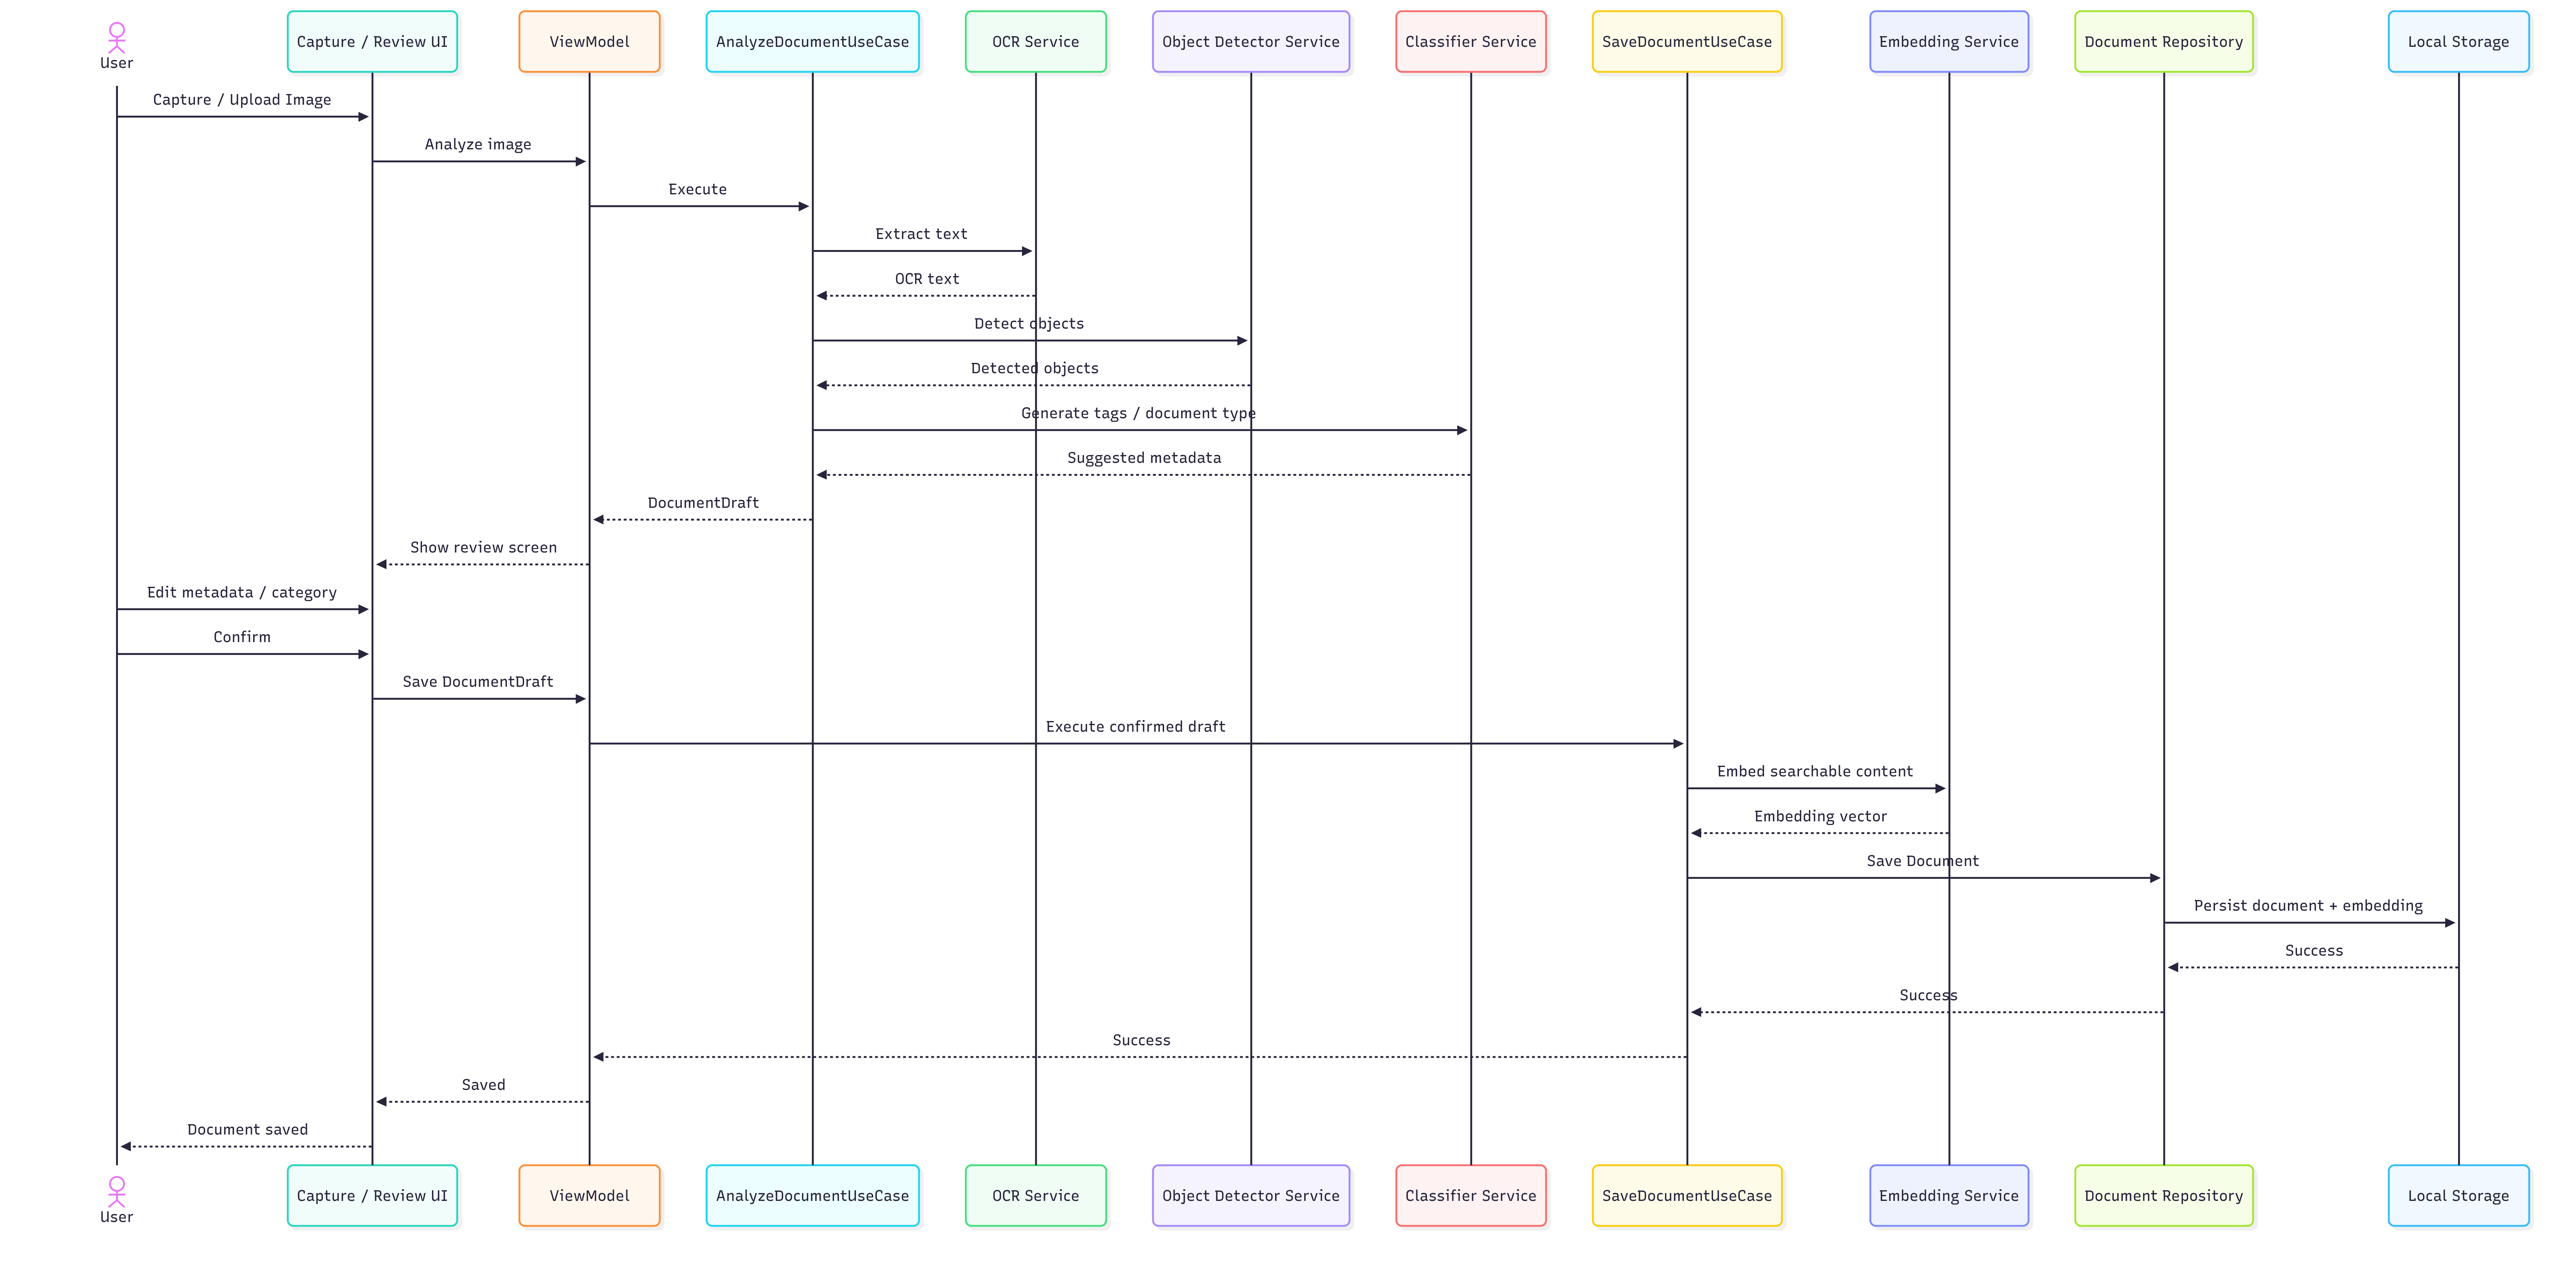
\includegraphics[width=\textwidth]{figures/AnalyzeFlow.png}
\caption{Document analysis flow}
\label{fig:seq_capture_save}
\end{figure}

\subsubsection{Hybrid Search Flow}
The sequence below traces a real-time search query from user keystroke debouncing to embedding generation, similarity ranking, and reactive UI updates:

\begin{figure}[H]
\centering
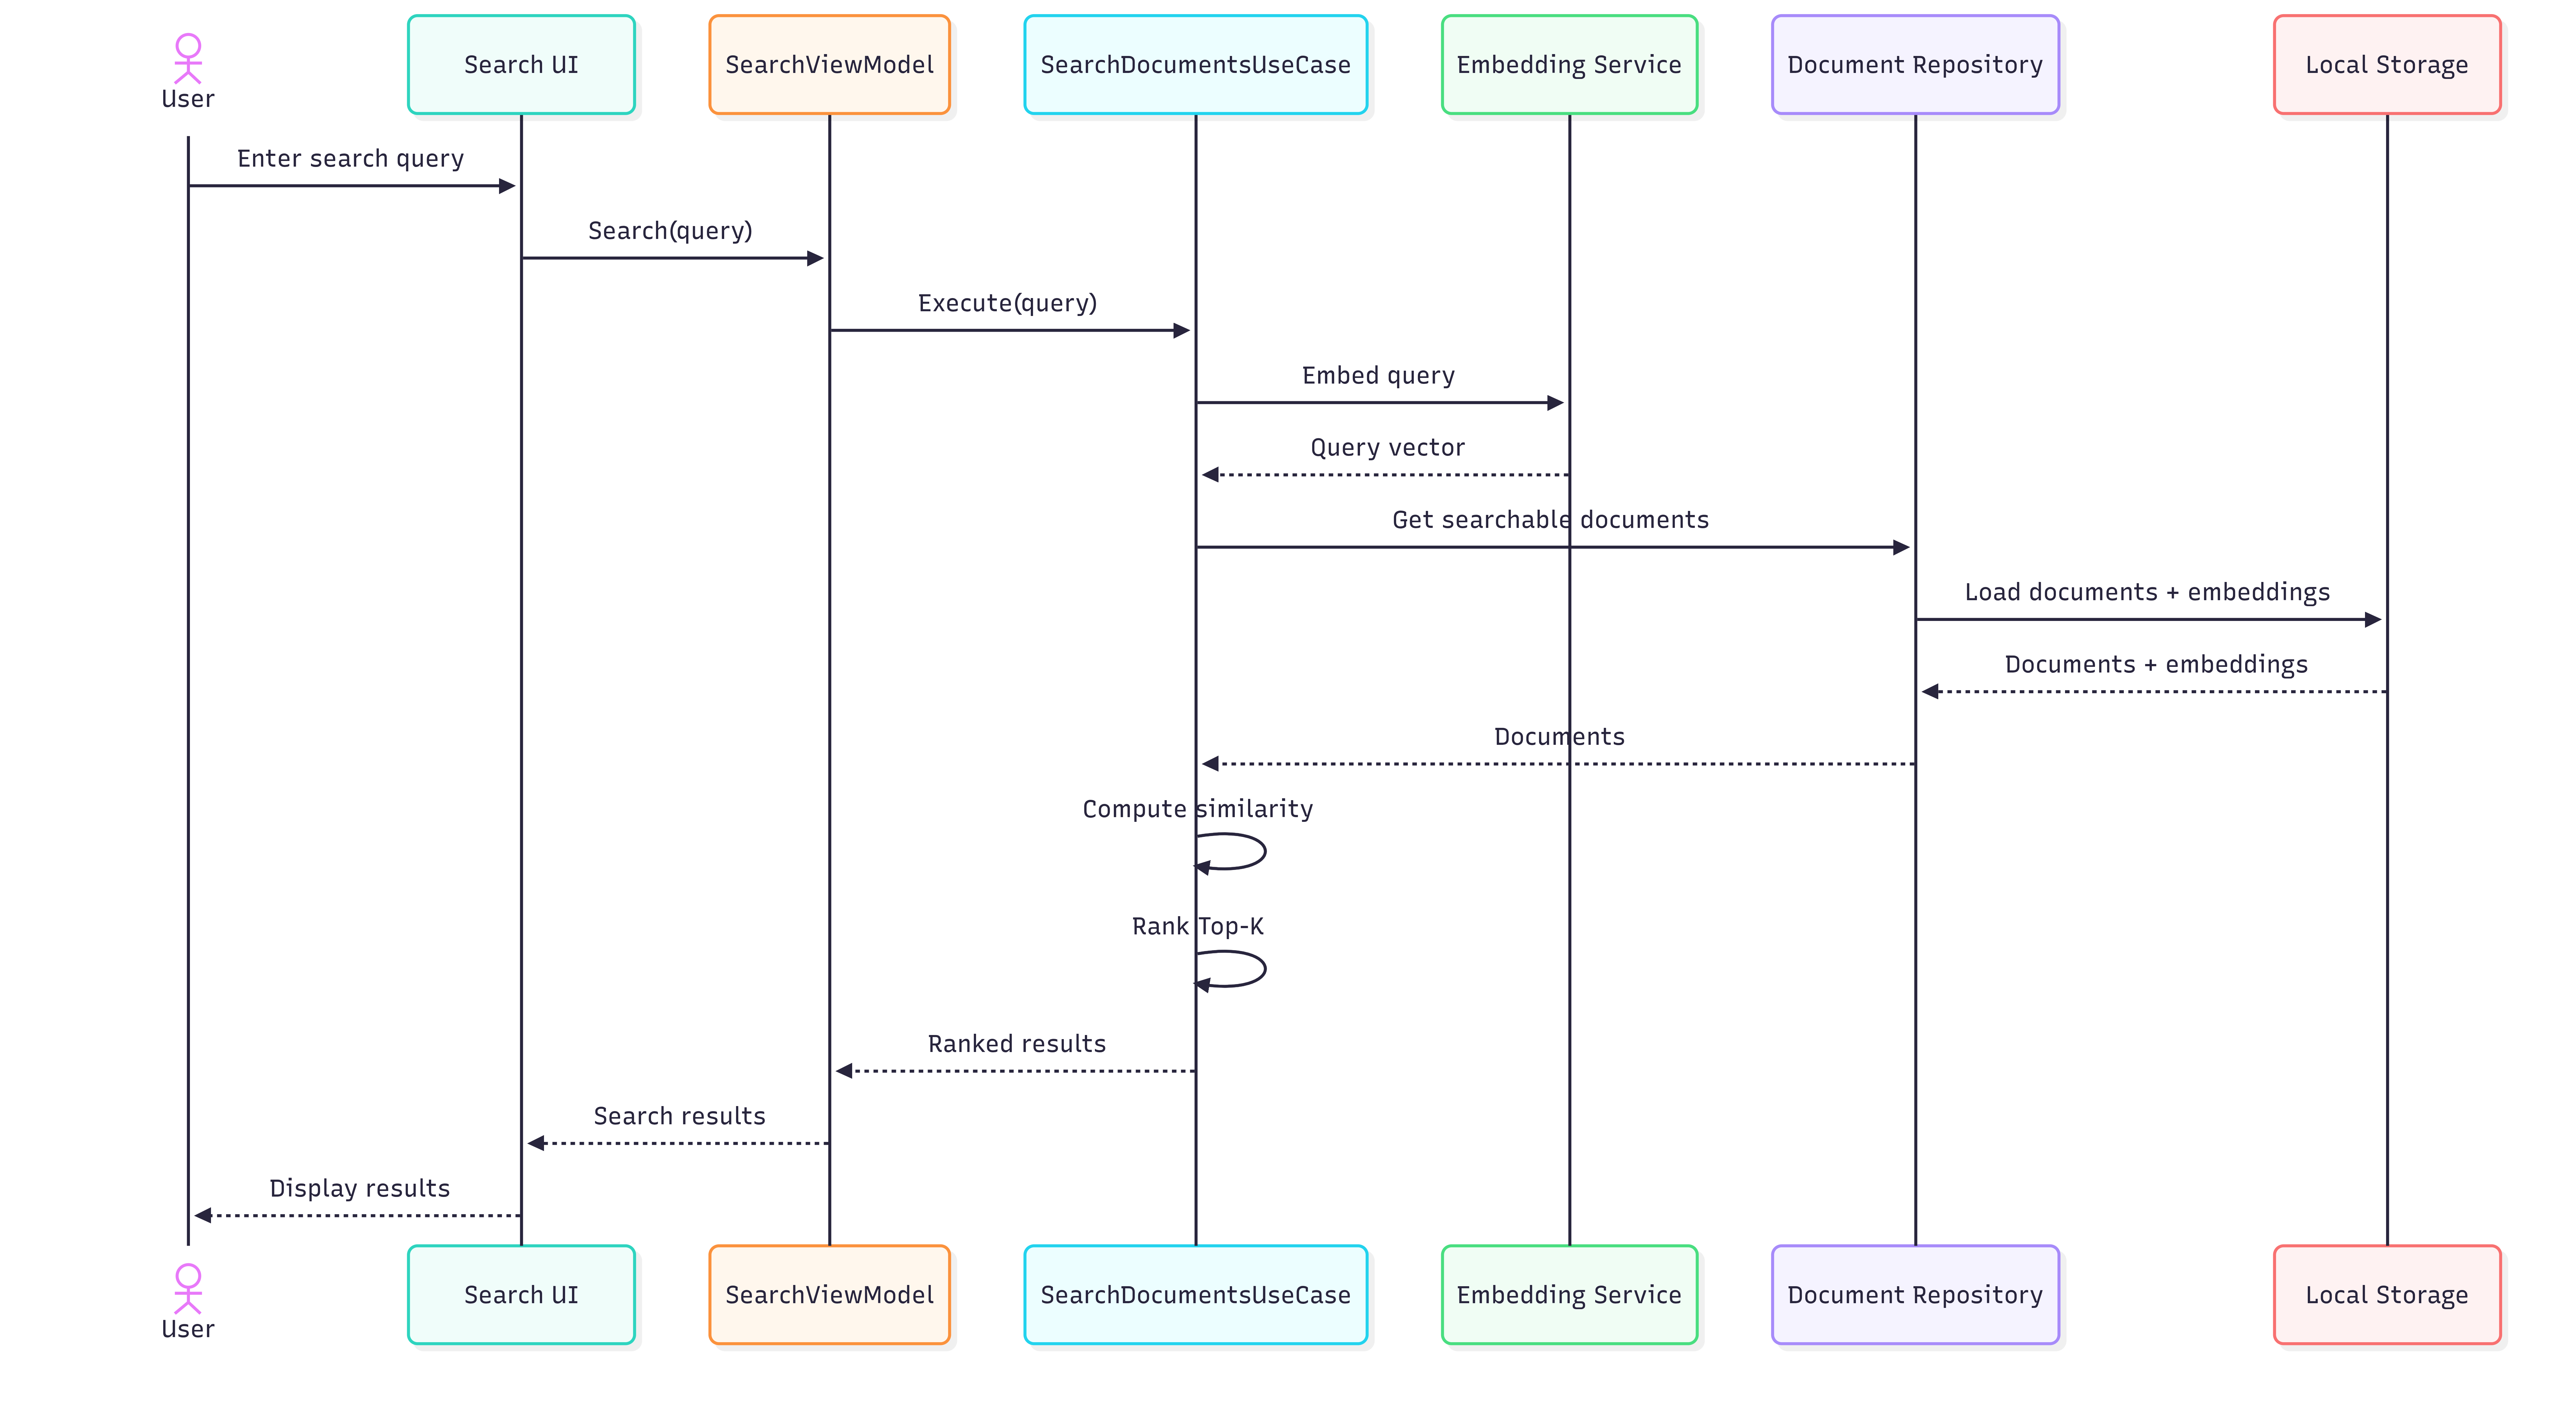
\includegraphics[width=\textwidth]{figures/SearchFlow.png}
\caption{Hybrid search flow}
\label{fig:seq_search}
\end{figure}


\section{Technical Implementation}

\subsection{Functional Pipeline}
The core operational lifecycle of the system operates in a continuous, end-to-end loop:
\begin{center}
\small
\textbf{Input Image} $\longrightarrow$ \textbf{Extract Metadata} $\longrightarrow$ \textbf{Vector Embedding} $\longrightarrow$ \textbf{Retrieval and Ranking}
\end{center}

To balance high-accuracy reasoning with offline resilience, the application follows a \textbf{Cloud-First with On-Device Fallback} paradigm comprising two interchangeable execution branches:

\subsubsection{Online Processing Pipeline}
When the device possesses active internet connectivity and an authorized API key is configured (\texttt{BuildConfig.GEMINI\_API\_KEY}), the application prioritizes Google's \textbf{Gemini 3.1 Flash Lite} (or \textbf{Gemini 3.1 Flash}) multimodal model managed by \texttt{GeminiApiLlmService}.

\paragraph{Execution Process:}
The raw image is read from local storage into a byte array (\texttt{ByteArray}) and dispatched alongside a structured prompt instructing the model to act as an advanced document analysis assistant. 

The LLM is constrained to respond with \textbf{ONLY a valid JSON object} (excluding code fences or narrative commentary) adhering strictly to the typed schema:

\begin{lstlisting}[language=json, caption={Structured JSON response schema returned by Gemini Vision API}]
{
  "title": "Short human-readable title (max 60 characters)",
  "description": "One concise sentence summarising what the document contains",
  "ocrText": "Full plain text read or extracted from the document image",
  "category": "NOTE | RECEIPT | IDENTITY | STUDY | WORK | OTHER",
  "tags": [
    "keyword1", 
    "keyword2", 
    "keyword3", 
    "keyword4", 
    "keyword5"
  ],
  "detectedObjects": [
    "paper", 
    "document", 
    "receipt"
  ]
}
\end{lstlisting}

\paragraph{Core Advantages:}
Leveraging large multimodal parameters, Gemini effortlessly deciphers skewed text orientations, low-contrast scans, handwritten notes, and irregular receipt layouts, yielding top-tier semantic categorization and contextual summaries.

\subsubsection{Offline Processing Pipeline}
Whenever network calls time out, encounter HTTP quota limits, or when the user explicitly toggles the \textbf{"Disable API"} setting in \texttt{SettingScreen}, the system seamlessly activates the local on-device ML suite:

\begin{enumerate}[label=\textbf{4.1.\arabic*.}]
    \item \textbf{OCR Service (Google ML Kit Text Recognition):}
    \begin{itemize}
        \item Implemented in \texttt{MlKitOcrService}.
        \item Uses Google ML Kit's Latin script text recognizer operating entirely on-device (leveraging NNAPI/GPU hardware acceleration when available).
        \item Extracts bounding text blocks, lines, and tokens from the bitmap without transmitting any data over the network.
    \end{itemize}

    \item \textbf{Image Labeling / Object Detection (Google ML Kit):}
    \begin{itemize}
        \item Implemented in \texttt{MlKitImageLabelingService}.
        \item Utilizes \texttt{ImageLabeling.getClient} configured with a confidence threshold $\ge 0.70$.
        \item Detects prominent physical items (e.g., \textit{Paper, Document, Receipt, Book, Invoice, Signature}) to support semantic classification.
    \end{itemize}

    \item \textbf{Description Generation Service (Google MediaPipe Tasks):}
    \begin{itemize}
        \item Implemented in \texttt{MediaPipeDescriptionGenerationService}.
        \item Employs the \textbf{MediaPipe Text Summarizer} model executing locally in \texttt{TLDR} mode (\texttt{MAX\_NUM\_TOKENS = 64}).
        \item The model binary is pre-bundled within \texttt{assets/} and copied to the internal application cache for instantaneous inference.
        \item Formulates a coherent single-sentence overview summarizing the OCR text and detected objects.
    \end{itemize}

    \item \textbf{Tag Generation Service:}
    \begin{itemize}
        \item Implemented in \texttt{SimpleTagGenerationService}.
        \item Fuses object labels with salient tokens filtered from the OCR transcription.
        \item \textbf{Bilingual Stop-Word Filtering:} Strips irrelevant tokens across English (\textit{the, and, for, with...}) and Vietnamese (\textit{cua, va, la, cac, trong, cho, ngay, thang, nam...}).
        \item \textbf{Domain Keyword Prioritization:} Elevates high-value domain tokens (\textit{receipt, invoice, passport, identity, license, certificate, contract, lecture, homework, report, project}).
        \item Computes word occurrence frequencies to select the top 5 most representative tags.
    \end{itemize}

    \item \textbf{Category Classification Service (Semantic Category Matching):}
    \begin{itemize}
        \item Implemented in \texttt{EmbeddingCategoryClassificationService}.
        \item Defines dense semantic anchor descriptions for standard target categories:
        \begin{itemize}
            \item \texttt{NOTE}: \textit{"personal note, memo or reminder"}
            \item \texttt{RECEIPT}: \textit{"receipt, invoice, purchase, payment, subtotal, or total"}
            \item \texttt{IDENTITY}: \textit{"passport, id card, driving license, official identification, certificate"}
            \item \texttt{STUDY}: \textit{"lecture notes, textbook, exam, homework, course, syllabus, student"}
            \item \texttt{WORK}: \textit{"meeting notes, project plan, contract, business report, presentation, employment"}
        \end{itemize}
        \item Embeds these category definitions into 512-dimensional vector space using \texttt{MediaPipeEmbeddingService}.
        \item During document classification, the aggregated document text is vectorized and matched against category embeddings using \textbf{Cosine Similarity}. The category yielding the highest score above $0.30$ is assigned; otherwise, the document defaults to \texttt{OTHER}.
    \end{itemize}
\end{enumerate}

\subsubsection{Metadata Review}
A crucial architectural decision is that \textbf{no raw AI output is saved directly into the database}:
\begin{itemize}
    \item Output fields from Gemini or the local ML pipeline are bundled into an immutable \textbf{\texttt{DocumentDraft}}.
    \item The user is automatically transitioned to \textbf{\texttt{ReviewScreen}}, where they are presented with the captured image alongside the pre-filled metadata.
    \item Users maintain complete authority to edit titles, adjust summaries, correct misclassified categories, or add/delete tags via interactive Material 3 chips.
    \item \textbf{Final Persistence:} Only when the user taps \textbf{"Confirm/Save"} is the finalized metadata synthesized into a searchable document string:
    $$\text{searchableText} = \text{title} + \text{description} + \text{ocrText} + \text{tags} + \text{detectedObjects}$$
    This consolidated string is vectorized by \texttt{MediaPipeEmbeddingService} and stored alongside the document record in Room Database.
\end{itemize}

\subsubsection{Hybrid Search Engine}
Search queries initiated on \texttt{LibraryScreen} utilize a hybrid ranking formulation balancing conceptual understanding with textual precision:
\begin{equation}
\text{TotalScore} = 0.8 \times \text{SemanticScore} + 0.2 \times \text{LexicalScore}
\end{equation}

\paragraph{1. Semantic Vector Score:}
Determined by cosine similarity between the query embedding vector and the stored document vector, which measures the degree of alignment between their vector directions.

\paragraph{2. Fuzzy Lexical Score:}
To accommodate spelling typos (e.g., searching \textit{"databse"} instead of \textit{"database"}), the system computes a normalized similarity based on the Levenshtein edit distance:
\begin{equation}
\text{fuzzySimilarity}(a, b) = 
\begin{cases}
1.0 & \text{if } \max(|a|, |b|) = 0 \\
1.0 - \dfrac{\text{levenshteinDistance}(a, b)}{\max(|a|, |b|)} & \text{otherwise}
\end{cases}
\end{equation}

Given query terms $Q$ and document terms $D$, the aggregate lexical score represents the mean of each query term's maximum similarity:
\begin{equation}
\text{LexicalScore} = \frac{1}{|Q|} \sum_{q \in Q} \left( \max_{d \in D} \text{fuzzySimilarity}(q, d) \right)
\end{equation}

\paragraph{3. Dual-Threshold Result Filtering:}
Documents are retained in the search results if and only if they satisfy the dual-threshold condition:
\begin{equation}
\text{Retain} \iff \left( \text{TotalScore} \ge 0.25 \right) \;\lor\; \left( \text{LexicalScore} \ge 0.50 \right)
\end{equation}
This rule ensures that strong semantic matches are surfaced even when exact wording differs, while near-identical lexical matches (e.g., misspelled keywords with LexicalScore $\ge 0.50$) are preserved even if semantic embeddings yield a modest score.

\subsection{User Interface and Navigation}

The application comprises five cohesive screens orchestrated through \texttt{AppNavGraph}:

\begin{figure}[H]
\centering
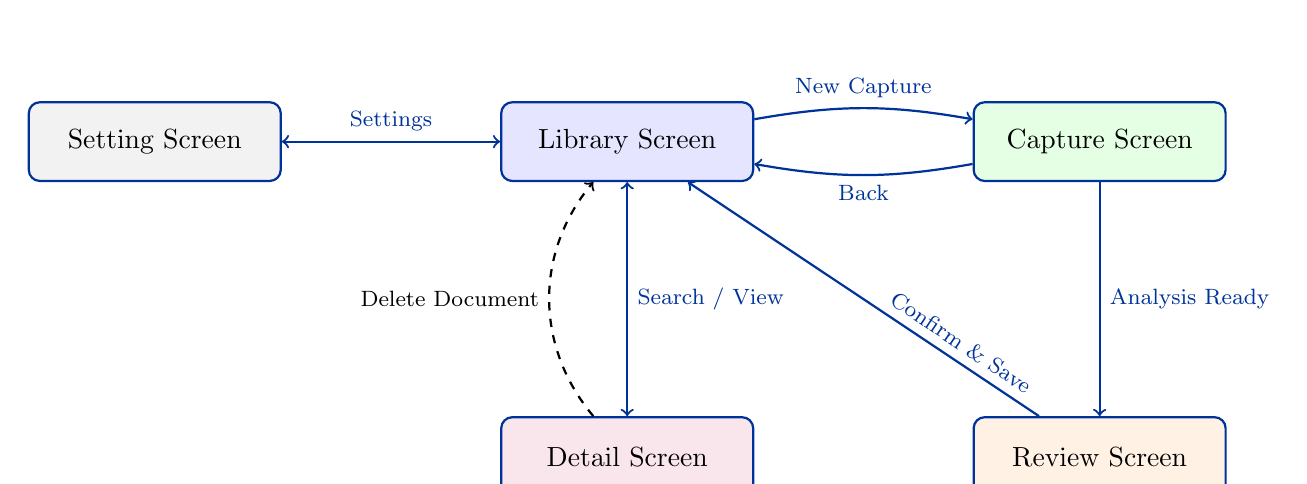
\begin{tikzpicture}[node distance=2.5cm, auto]
    % Screen nodes
    \node[draw=deepblue, fill=blue!10, rounded corners, thick, minimum width=3.2cm, minimum height=1cm] (lib) {Library Screen};
    \node[draw=deepblue, fill=green!10, rounded corners, thick, right of=lib, xshift=3.5cm, minimum width=3.2cm, minimum height=1cm] (cap) {Capture Screen};
    \node[draw=deepblue, fill=orange!10, rounded corners, thick, below of=cap, yshift=-1.5cm, minimum width=3.2cm, minimum height=1cm] (rev) {Review Screen};
    \node[draw=deepblue, fill=purple!10, rounded corners, thick, below of=lib, yshift=-1.5cm, minimum width=3.2cm, minimum height=1cm] (det) {Detail Screen};
    \node[draw=deepblue, fill=gray!10, rounded corners, thick, left of=lib, xshift=-3.5cm, minimum width=3.2cm, minimum height=1cm] (set) {Setting Screen};

    % Transitions
    \draw[<->, thick, deepblue] (lib) -- node[right]{\footnotesize Search / View} (det);
    \draw[->, thick, deepblue] (lib) to[bend left=10] node[above]{\footnotesize New Capture} (cap);
    \draw[->, thick, deepblue] (cap) to[bend left=10] node[below]{\footnotesize Back} (lib);
    \draw[->, thick, deepblue] (cap) -- node[right]{\footnotesize Analysis Ready} (rev);
    \draw[->, thick, deepblue] (rev) -- node[sloped, above, pos=0.25]{\footnotesize Confirm \& Save} (lib);
    \draw[<->, thick, deepblue] (lib) -- node[above]{\footnotesize Settings} (set);
    \draw[->, thick, dashed] (det) to[bend left=40] node[left]{\footnotesize Delete Document} (lib);
\end{tikzpicture}
\caption{Screen navigation state graph (App Navigation Flow)}
\label{fig:app_nav}
\end{figure}

\begin{enumerate}
    \item \textbf{LibraryScreen (Primary Repository \& Live Search):}
    \begin{itemize}
        \item Entry point displaying stored items in a responsive grid/list view (\texttt{DocumentCard}).
        \item Top search bar featuring a 100ms debounce delay for fluent, stutter-free real-time queries.
        \item Displays category badges, topical tags, creation dates, and debug score badges (\texttt{sem: xxx}, \texttt{lex: xxx}).
    \end{itemize}

    \item \textbf{CaptureScreen (Document Capture \& Media Import):}
    \begin{itemize}
        \item Integrates CameraX for fast auto-focus and tap-to-focus document imaging.
        \item Supports importing pre-existing document images from device storage via the Android Photo Picker.
    \end{itemize}

    \item \textbf{ReviewScreen (Human-in-the-Loop Inspection \& Editing):}
    \begin{itemize}
        \item Renders captured imagery alongside AI-inferred suggestions.
        \item Displays a prominent fallback warning banner if the cloud API failed and on-device fallback was used.
        \item Provides editable text fields and category selector chips for user adjustments before final database commit.
    \end{itemize}

    \item \textbf{DetailScreen (Full Document Inspection \& Zoom Viewer):}
    \begin{itemize}
        \item Presents complete metadata, transcribed OCR text blocks, and timestamps.
        \item Integrates \texttt{FullScreenImageViewer} with two-finger pinch-to-zoom and pan gestures.
        \item Facilitates document editing or deletion with atomic storage cleanup.
    \end{itemize}

    \item \textbf{SettingScreen (System Configuration \& Diagnostics):}
    \begin{itemize}
        \item \textbf{API Toggle:} Allows users to disable external API calls to enforce complete offline privacy.
        \item \textbf{Camera Start Mode:} Option to launch directly into the capture view upon app startup.
        \item \textbf{Factory Reset:} Wipes Room Database records, DataStore preferences, and internal image caches to restore initial state.
    \end{itemize}
\end{enumerate}

\section{Future Work and Technical Roadmap}

\subsection{On-Device Language Models}
The current \textbf{Cloud-First with Local Fallback} architecture delivers a dependable balance between multimodal precision and continuous offline utility. Nevertheless, empirical usage highlights distinct limitations when operating strictly offline:
\begin{itemize}
    \item \textbf{Heuristic OCR Limitations on Unstructured Media:} Traditional mobile OCR engines (such as ML Kit Text Recognition) perform exceptionally well on high-contrast printed typography, but experience noticeable degradation when parsing freehand handwriting, skewed receipt margins, faint inks, or intricate tabular matrices.
    \item \textbf{Cascading Metadata Degradation:} Because downstream tasks (title generation, text summarization, category classification, and keyword tagging) rely upon OCR tokens, noisy optical transcription directly degrades downstream accuracy, requiring heavier user manual corrections on the Review screen.
\end{itemize}

\paragraph{Prospective Architectural Evolution:}
Directly embedding quantized \textbf{Small Language Models (SLMs)} within the local mobile runtime via Google MediaPipe GenAI SDK, ONNX Runtime Mobile, or ExecuTorch. Candidate models include:
\begin{itemize}
    \item \textbf{Google Gemma 2B / Gemma-4N:} Tailored for mobile acceleration on modern NPU and GPU architectures.
    \item \textbf{Qwen 2.5 (0.5B / 1.5B):} Exceptionally compact footprint, rapid token generation, and robust multilingual comprehension (particularly English and Vietnamese).
    \item \textbf{LLaMA-3.2 1B/3B Mobile:} 4-bit integer quantization (\textit{INT4}) enabling execution within mobile thermal envelopes.
\end{itemize}

\paragraph{Hardware Constraints and Pragmatic Trade-offs:}
While on-device SLMs are technically compelling, mobile devices in entry-level segments with limited RAM ($\le 4\text{GB}$) risk severe Out-Of-Memory (OOM) exceptions and thermal throttling when allocating 1.5GB to 3GB model weights into working memory. Consequently, the optimal architectural roadmap involves a \textbf{Dynamic Hardware Capability Detector}: devices equipped with ample RAM ($\ge 8\text{GB}$) and dedicated NPUs will execute local SLMs, while standard devices will continue leveraging the lightweight ML Kit and MediaPipe Embedder pipeline.

\subsection{Feature Extensions}

\subsubsection{Repository Question Answering}
A natural extension of semantic search is upgrading from ranked retrieval to full \textbf{Retrieval-Augmented Generation (RAG)} across the user's personal document collection (analogous to an on-device personal NotebookLM):
\begin{itemize}
    \item Enabling conversational queries over multi-document contexts:
    \begin{itemize}
        \item \textit{"What was my total expenditure on client lunches last month?"}
        \item \textit{"When does my air conditioner warranty expire?"}
        \item \textit{"Summarize all key formulas from the database indexing lecture."}
    \end{itemize}
    \item \textbf{Feasibility Assessment:} While technically promising, multi-document synthesis requires significant vector ranking pipelines and context management. In alignment with the project's primary objective---providing instantaneous retrieval for forgetful users with zero lag---this capability is prioritized for subsequent major revisions.
\end{itemize}

\subsubsection{Deadline and Follow-Up Notifications}
Physical documents frequently involve critical temporal triggers:
\begin{itemize}
    \item Utility bills and credit card statements requiring settlement by a specific calendar date.
    \item Saved articles, technical tutorials, or reading materials captured for weekend review.
    \item Medical follow-up appointments, passport renewal milestones, or flight departures.
\end{itemize}

\paragraph{Proposed Implementation:}
Integrating an on-device \textbf{Temporal Entity Extractor} within the metadata pipeline. Upon detecting payment deadlines or appointment dates:
\begin{itemize}
    \item The system automatically prompts the user to schedule a local reminder.
    \item Leverages Android's \texttt{AlarmManager} and \texttt{WorkManager} to dispatch reliable local notifications (\textit{Local Push Notifications}) without needing external push notification servers.
\end{itemize}

\section{Self-Assessment}

This project was completed as a collaborative Android application development effort aimed at solving a realistic personal-document management problem. Overall, we believe the system successfully meets the core requirements of the course: it is implemented as a native Android application with multiple connected screens, persistent local storage, and integrated AI/ML-based document-processing features. The app supports image capture or import, automatic OCR and metadata extraction, classification, search, and review before persistence.

\paragraph{What we completed successfully:}
\begin{itemize}
    \item The app provides a dedicated personal document library separated from the system gallery, allowing safe and organized storage of scanned or captured documents.
    \item The pipeline for document analysis works in both online and offline modes. The online mode leverages Gemini for richer multimodal analysis, while the offline mode relies on local ML Kit and MediaPipe components to ensure functional availability without internet access.
    \item The application includes a hybrid search system that combines semantic embedding similarity with fuzzy lexical matching, improving recall when the user remembers only approximate phrases or misspelled keywords.
    \item The UI was designed to support a clear user flow from capture, to review, to storage, and then to search or detail inspection.
    \item The project follows a clean separation between presentation, domain logic, and data infrastructure, which makes the codebase more maintainable and easier to extend.
\end{itemize}

\paragraph{What we improved and learned:}
\begin{itemize}
    \item We strengthened our understanding of Android architecture patterns, especially MVVM, Flow-based state handling, Room persistence, and dependency injection through a custom container.
    \item We learned how to integrate AI/ML capabilities into mobile workflows while balancing accuracy, efficiency, and privacy requirements.
    \item We improved our ability to design an app around real user pain points, focusing not only on visual interface quality but also on practical retrieval and organization workflows.
\end{itemize}

\paragraph{Current limitations:}
\begin{itemize}
    \item The system is designed as a single-user personal repository rather than a collaborative or multi-device platform.
    \item In fully offline conditions, document accuracy can still depend on OCR quality and local model limitations, especially for handwritten or highly distorted content.
    \item The system currently focuses on local document management and retrieval rather than full multi-document reasoning or advanced RAG-style question answering.
\end{itemize}

\paragraph{Overall assessment:}
We consider the project to be a successful capstone implementation for the course. It demonstrates both technical depth and practical value, combining Android development, local persistence, AI/ML processing, and user-centered design in a working application. The project not only meets the course's functional expectations but also provides a solid foundation for future extensions such as richer document understanding, reminders, and expanded personal knowledge retrieval.


\section{References}
\begin{itemize}
    \item Martin, Robert C. \textit{Clean Architecture: A Craftsman's Guide to Software Structure and Design}. Prentice Hall.
    \item Google Developers. \textit{Guide to app architecture}. Android Developers Documentation. Available at: \url{https://developer.android.com/topic/architecture}
    \item Google Developers. \textit{Jetpack Compose documentation}. Android Developers Documentation. Available at: \url{https://developer.android.com/jetpack/compose}
    \item Android Developers. \textit{Android documentation}. Available at: \url{https://developer.android.com/}
    \item Google ML Kit. \textit{ML Kit documentation}. Available at: \url{https://developers.google.com/ml-kit}
    \item Google MediaPipe. \textit{MediaPipe documentation}. Available at: \url{https://developers.google.com/mediapipe}
    \item Google AI for Developers. \textit{Gemini API documentation}. Available at: \url{https://ai.google.dev/gemini-api/docs}
\end{itemize}

\end{document}
